\section{Part I: Data Cleaning and Preprocessing (for dataset A)}
\subsection{Detecting Issues in the dataset}
For this part of the assignment, the dataset had to be analyzed first to detect issues such as missing values and outliers. There was found to be a 124053 missing values and 14622 outliers.  

\subsection{Fixing Issues}
Before replacing the missing values with the mean, the outliers had to be checked first since the mean would be effected by the outliers. To find the outliers, the standard deviation of the values was determined first and used to find values that vary by more than 3 standard deviations. There were over 14000 data points that vary from the features mean by over 3 standard deviations. Those outlier values were replace with the mean of each feature. Final step was to replace all the missing values with the mean after the outliers were taken care of. 


\subsection{Normalizing Data}

Figure~\ref{fig:fig1} shows the comparison between histogram plots of feature 9 and 24 before and after normalization

%%%%%%%%%%%%%%%%%%%%%%%%%%%%%%%%%%%%%%%%%%%%%%%%%%%%%%%%%%%%%%%%%%%
%
% Commands to include a figure:
%
%%%%%%%%%%%%%%%%%%%%%%%%%%%%%%%%%%%%%%%%%%%%%%%%%%%%%%%%%%%%%%%%%%%

\begin{figure}[!ht]
 \centering
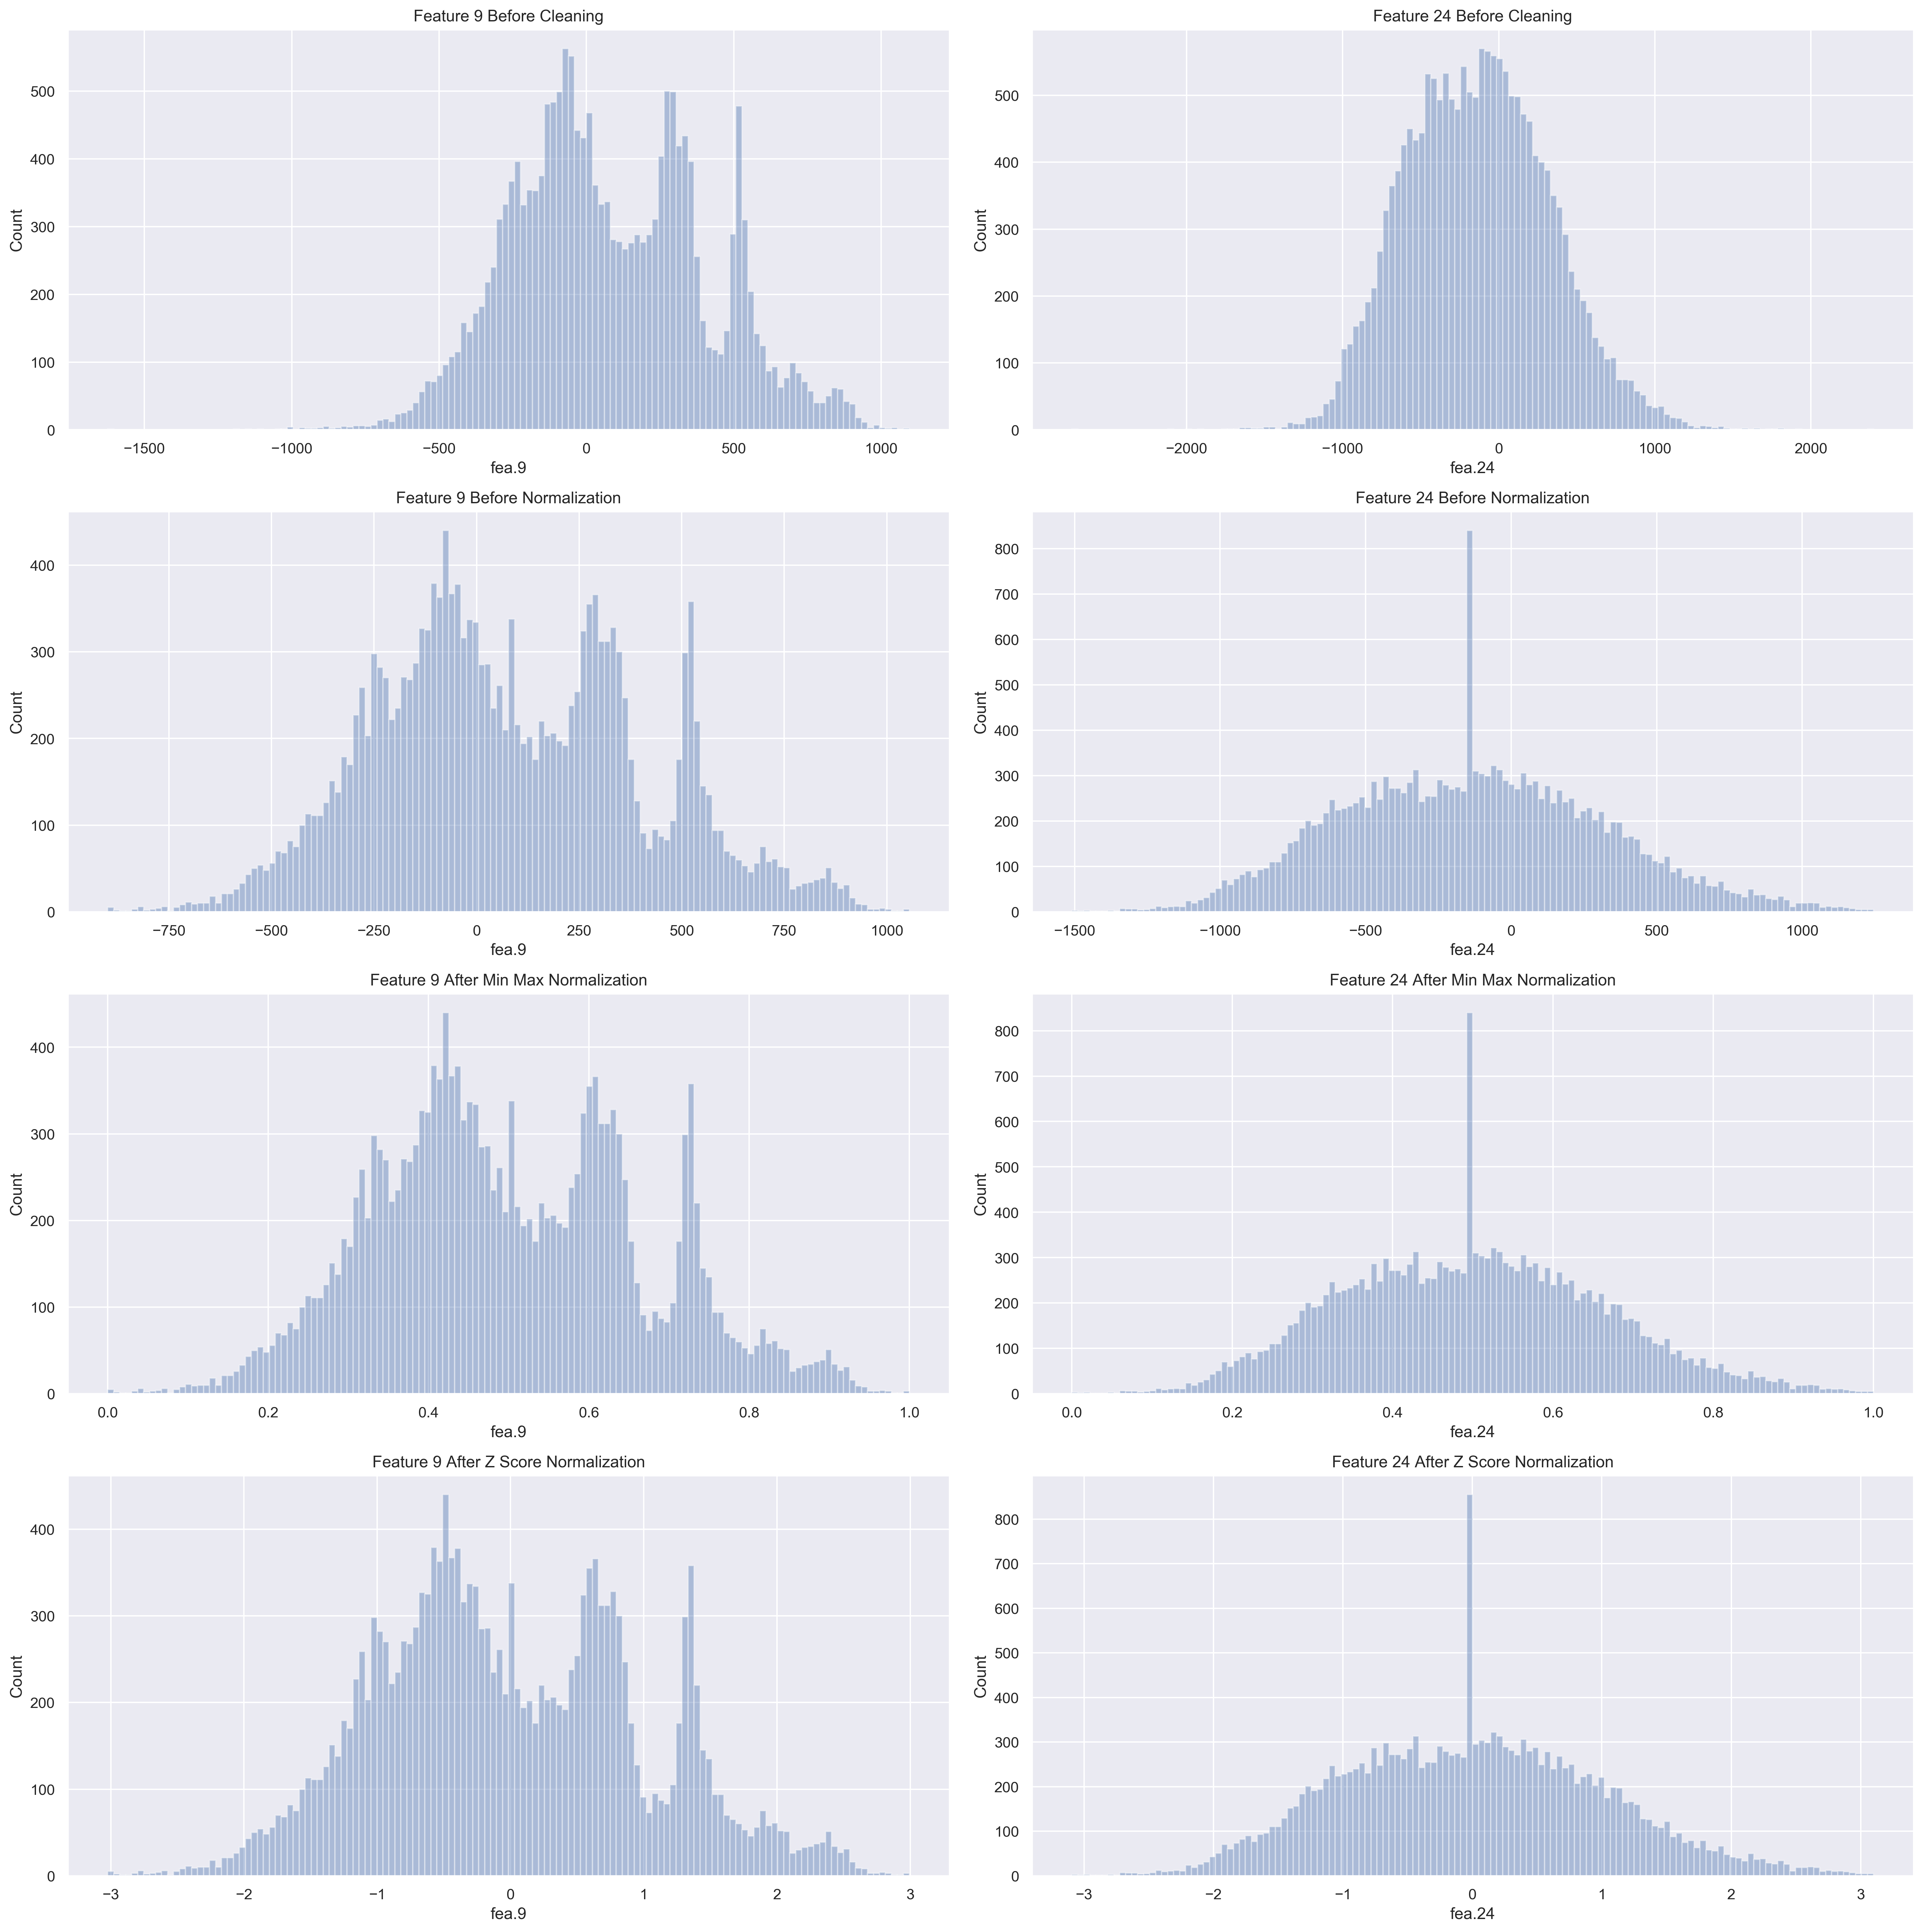
\includegraphics[width=6.1in]{assignment1/1-3-histograms.png}
\caption{\label{fig:fig1}histogram plots of feature 9 and 24 before and after normalization}
\end{figure}
